\documentclass{math}

\usepackage{tikz}

\title{University Physics 1A}
\author{Alvin Lin}
\date{December 7th, 2017}

\begin{document}

\maketitle

\section*{Waves}
\begin{center}
  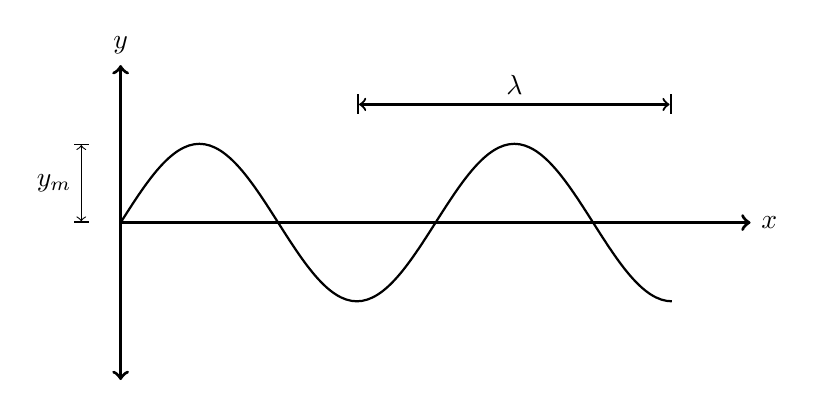
\begin{tikzpicture}
    \draw[<->,very thick] (0,-2) -- (0,2) node[above] {\( y \)};
    \draw[->,very thick] (0,0) -- (8,0) node[right] {\( x \)};
    \draw[thick] (0,0) sin (1,1) cos (2,0) sin (3,-1) cos (4,0) sin (5,1) cos (6,0) sin (7,-1);
    \draw[|<->|,thick] (3,1.5) -- (7,1.5) node[pos=0.5,above] {\( \lambda \)};
    \draw[|<->|] (-0.5,0) -- (-0.5,1) node[pos=0.5,left] {\( y_m \)};
  \end{tikzpicture}
    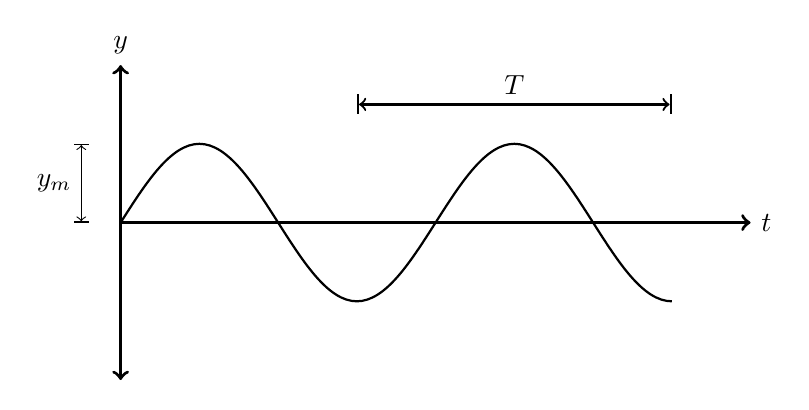
\begin{tikzpicture}
      \draw[<->,very thick] (0,-2) -- (0,2) node[above] {\( y \)};
      \draw[->,very thick] (0,0) -- (8,0) node[right] {\( t \)};
      \draw[thick] (0,0) sin (1,1) cos (2,0) sin (3,-1) cos (4,0) sin (5,1) cos (6,0) sin (7,-1);
      \draw[|<->|,thick] (3,1.5) -- (7,1.5) node[pos=0.5,above] {\( T \)};
      \draw[|<->|] (-0.5,0) -- (-0.5,1) node[pos=0.5,left] {\( y_m \)};
    \end{tikzpicture}
\end{center}
A wave pattern moves \( \lambda \) in \( T \).
\[ T = \frac{1}{f} \]
\[ v = \frac{\text{how far it goes}}{\text{how long it takes}} =
  \frac{\lambda}{T} = \lambda f = \frac{\omega}{k} \]
The wave equation is of the form:
\[ y = y_m\cos(kx-\omega t) \]
with \( k \) the angular wave number in radians per meter and \( \omega \) the
angular frequency in radians per second.
\[ \omega = 2\pi f \]
\[ k = \frac{2\pi}{\lambda} \]
For a wave moving through a string, the speed of the wave is:
\[ v = \sqrt{\frac{tension}{mass~density}} =
  \sqrt{\frac{F_{tension}}{\lambda}} \]
Note that the lambda above represents mass density in kilograms per meter.

\subsection*{Wave Interference}
Two waves travelling in opposite directions with the same amplitude can be
represented as:
\[ y = 2y_m\sin(kx)\cos(\omega t) \]
\vspace{0.5cm}

\noindent\textbf{First harmonic (fundamental frequency):} \\
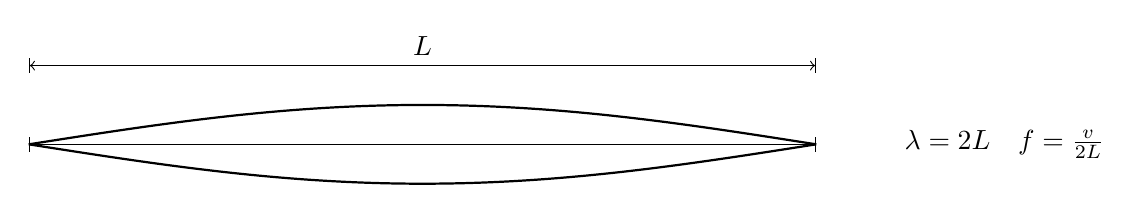
\begin{tikzpicture}
  \draw[|-|] (0,0) -- (10,0) node[right,xshift=1cm]
    {\( \lambda = 2L \quad f = \frac{v}{2L} \)};
  \draw[|<->|] (0,1) -- (10,1) node[pos=0.5,above] {\( L \)};
  \draw[thick] (0,0) sin (5,0.5) cos (10,0);
  \draw[thick] (0,0) sin (5,-0.5) cos (10,0);
\end{tikzpicture}
\vspace{1cm}

\noindent\textbf{Second harmonic (first overtone):} \\
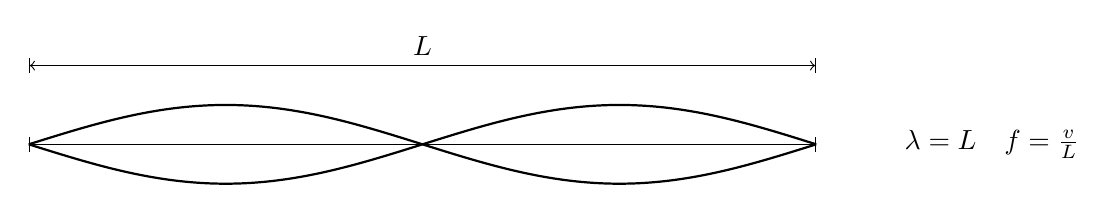
\begin{tikzpicture}
  \draw[|-|] (0,0) -- (10,0) node[right,xshift=1cm]
    {\( \lambda = L \quad f = \frac{v}{L} \)};
  \draw[|<->|] (0,1) -- (10,1) node[pos=0.5,above] {\( L \)};
  \draw[thick] (0,0) sin (2.5,0.5) cos (5,0) sin (7.5,-0.5) cos (10,0);
  \draw[thick] (0,0) sin (2.5,-0.5) cos (5,0) sin (7.5,0.5) cos (10,0);
\end{tikzpicture}
\vspace{1cm}

\noindent\textbf{Third harmonic (second overtone):} \\
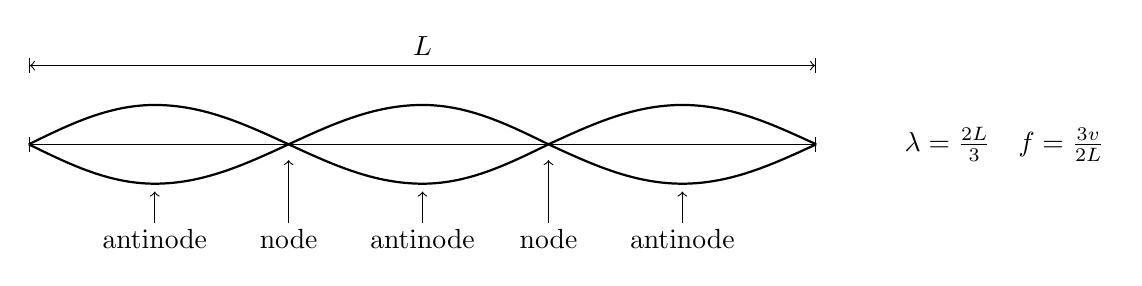
\begin{tikzpicture}
  \draw[|-|] (0,0) -- (10,0) node[right,xshift=1cm]
    {\( \lambda = \frac{2L}{3} \quad f = \frac{3v}{2L} \)};
  \draw[|<->|] (0,1) -- (10,1) node[pos=0.5,above] {\( L \)};
  \draw[thick] (0,0) sin (1.6,0.5) cos (3.3,0) sin (5,-0.5) cos (6.6,0)
    sin (8.3,0.5) cos (10,0);
  \draw[thick] (0,0) sin (1.6,-0.5) cos (3.3,0) sin (5,0.5) cos (6.6,0)
    sin (8.3,-0.5) cos (10,0);
  \draw[<-] (1.6,-0.6) -- (1.6,-1) node[yshift=-0.2cm] {antinode};
  \draw[<-] (3.3,-0.2) -- (3.3,-1) node[yshift=-0.2cm] {node};
  \draw[<-] (5,-0.6) -- (5,-1) node[yshift=-0.2cm] {antinode};
  \draw[<-] (6.6,-0.2) -- (6.6,-1) node[yshift=-0.2cm] {node};
  \draw[<-] (8.3,-0.6) -- (8.3,-1) node[yshift=-0.2cm] {antinode};
\end{tikzpicture}

\begin{center}
  You can find all my notes at \url{http://omgimanerd.tech/notes}. If you have
  any questions, comments, or concerns, please contact me at
  alvin@omgimanerd.tech
\end{center}

\end{document}
